\begin{frame}<1>[label=hookingList]{hooking}
    \begin{itemize}
    \item hooking --- getting a `hook' to run on (OS) operations
        \begin{itemize}
        \item e.g. creating new files
        \item e.g. modifying executable files
        \end{itemize}
    \item ideal mechanism: \myemph<2>{OS support}
    \item less ideal mechanism: \myemph<3>{change library loading}
        \begin{itemize}
        \item e.g. replace `open', `fopen', etc. in libraries
        \end{itemize}
    \item less ideal mechanism: \myemph<4>{replace OS exception} (system call) handlers
        \begin{itemize}
        \item very OS version dependent
        \end{itemize} 
    \item less ideal mechanism: \myemph<5>{debugger support}
    \end{itemize}
\end{frame}

\againframe<2>{hookingList}

\begin{frame}
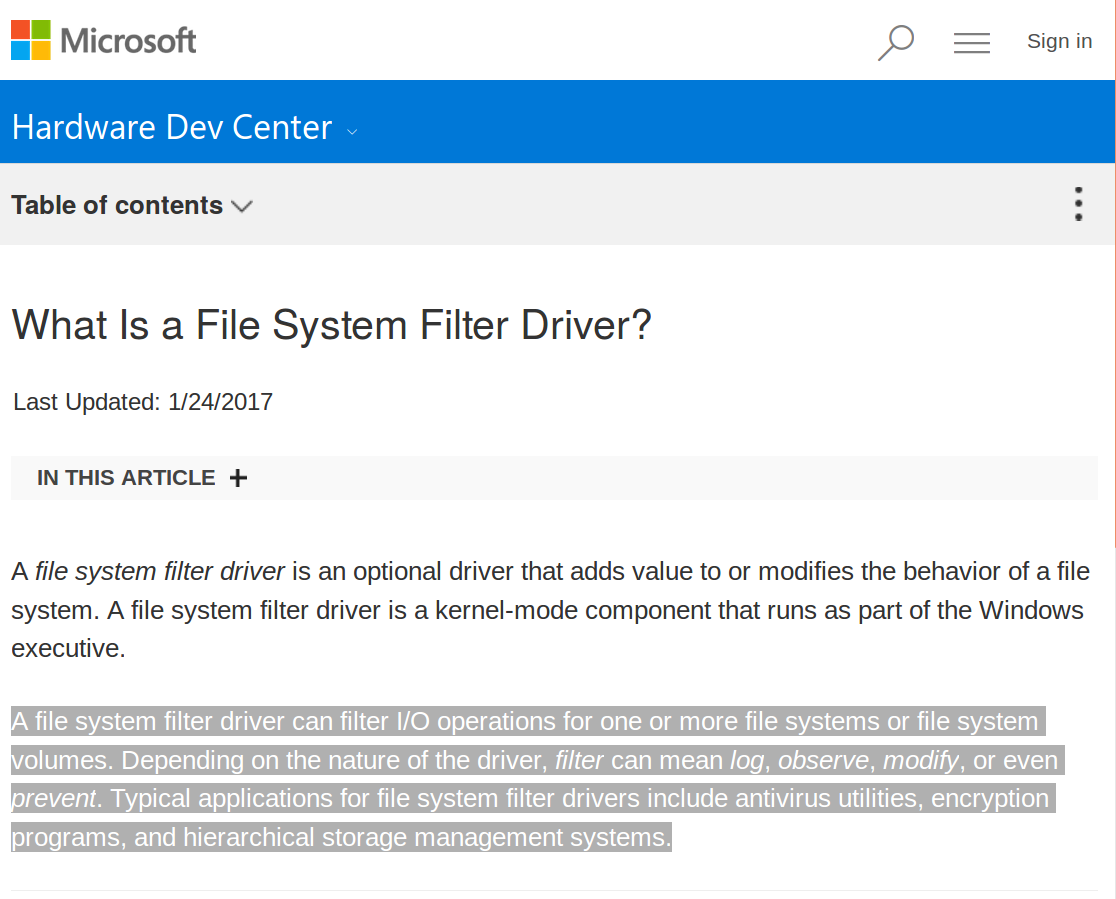
\includegraphics[height=0.9\textheight]{../antianti/filter-driver}
\end{frame}

\againframe<3>{hookingList}

\begin{frame}{changing library loading}
\begin{itemize}
    \item e.g. install new library --- or edit loader, but \ldots
    \vspace{.5cm}
    \item not everything uses library functions
    \item what if your wrapper doesn't work exactly the same?
\end{itemize}
\end{frame}

\againframe<4>{hookingList}

\begin{frame}{changing exception call handlers (1)}
    \begin{itemize}
    \item OS data structure tells hardware where program requests go
    \item simpliest mechanism: edit that data structure
       \begin{itemize}
       \item and save a copy of what was there before
       \end{itemize}
    \item point to your code
        \begin{itemize}
        \item and call what was there before after behavior check
        \end{itemize}
    \end{itemize}
\end{frame}

